\section*{Math 202A - Final Exam - Dan Davison - \texttt{ddavison@berkeley.edu}}

\begin{mdframed}
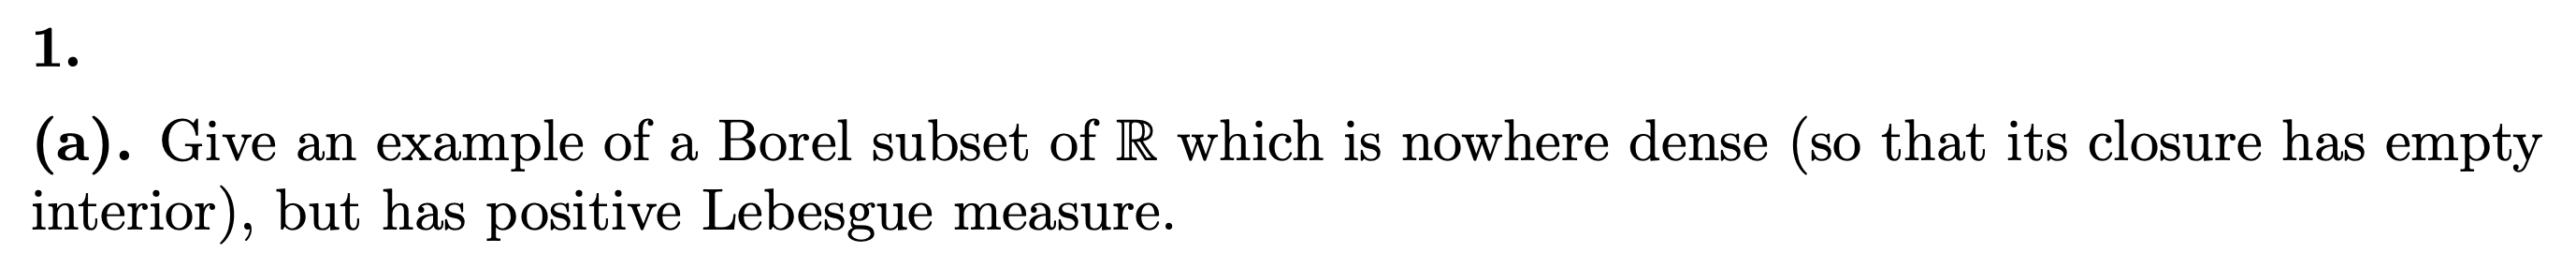
\includegraphics[width=400pt]{img/analysis--berkeley-202a-final-c9d2.png}
\end{mdframed}

\begin{proof}
  \green{DONE}

  The ``fat Cantor set​'' is an example of such a set. The fat Cantor set of measure $a \in (0, 1)$ is formed as
  follows:

  Note that $\sum_{n=1}^\infty \frac{1 - a}{2^n} = 1 - a$. So we will design an algorithm that
  removes $\frac{1-a}{2^n}$ at each iteration, for $n=1, 2, \ldots$. Note that at the start of iteration $n$
  there are $2^{n-1}$ intervals. So we remove
  \begin{align*}
    \frac{1-a}{2^{n}}\cdot\frac{1}{2^{n-1}} = \frac{1 - a}{2^{2n - 1}}
  \end{align*}
  from each interval.

  For example, to create a set with measure $a = \frac{1}{2}$,
  remove $\frac{1}{4} + 2(\frac{1}{16}) + 4(\frac{1}{64}) + \cdots = \frac{1}{2}$.
\end{proof}

\begin{mdframed}
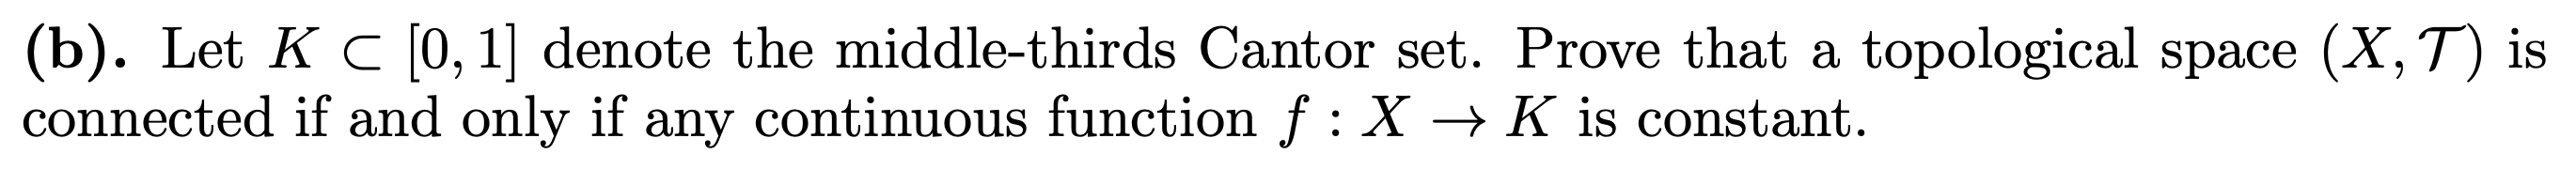
\includegraphics[width=400pt]{img/analysis--berkeley-202a-final-4333.png}
\end{mdframed}
\begin{lemma}\label{cantor-set-totally-disconnected}
  Let $k_1, k_2 \in K \subset \R$ with $k_1 \neq k_2$. Then $\{k_1\}$ and $\{k_2\}$ are connected subsets,
  and $[k_1, k_2]$ is disconnected.
\end{lemma}

\begin{proof}
  Let $k_1, k_2 \in K \subset \R$ with $k_1 \neq k_2$. Without loss of generality suppose that $k_1 < k_2$.
  Then there exists $x \in K^c$ such that $k_1 < x < k_2$ (\red{TODO} I hope we proved this in class?).
  Then $[k_1, x) \isect K$ and $(x, k_2] \isect K$ are non-empty open subsets of $K$ whose union
  equals $[k_1, k_2]$, therefore $[k_1, k_2]$ is disconnected.
\end{proof}

\begin{proof}
  \green{DONE}

  We view the middle-thirds Cantor set $K$ as a topological space with the topology induced by the standard
  metric on $\R$.

  $\implies$\\
  For the forwards implication, let $(X, \mc T)$ be a connected topological space and suppose for a
  contradiction that $f: X \to K$ is continuous but not constant.

  Then there exist $k_1, k_2 \in f(X)$ with $k_1 \neq k_2$. But from lemma
  \ref{cantor-set-totally-disconnected} we have that $[k_1, k_2]$ is disconnected. Therefore $f(X)$ is
  disconnected. But by Bass theorem 20.48 the image of a connected topological space under a continuous map
  between topological spaces is connected, and so this is a contradiction. Therefore if $f$ is continuous it
  must be constant.

  $\impliedby$\\
  For the reverse implication, let every continuous function $f: X \to K$ be constant and suppose for a
  contradiction that $(X, \mc T)$ is not connected.

  Let $G_1, G_2 \subset X$ be non-empty disjoint open subsets of $X$ such that $G_1 \union G_2 = X$.
  Let $H_1, H_2 \subset K$ be disjoint open subsets of $K$, and let $k_1 \in H_1$ and $k_2 \in H_2$. (\red{TODO}:
  prove that there are two disjoint open subsets of the Cantor set.)

  Define $f: X \to K$ by
  \begin{align*}
    f(x) =
    \begin{cases}
      k_1, & x \in G_1 \\
      k_2, & x \in G_2.
    \end{cases}
  \end{align*}
  Then $f$ is not constant. Furthermore, the preimage of every open subset of $K$ is open,
  since $f^{-1}(H_1) = G_1$ and $f^{-1}(H_2) = G_2$ and $f^{-1}(H) = \emptyset$ for every open subset $H$
  of $K$ such that $H \neq H_1$ and $H \neq H_2$. Therefore $f$ is continuous. This contradicts our premise and
  thus proves that $(X, \mc T)$ is connected.
\end{proof}

\begin{mdframed}
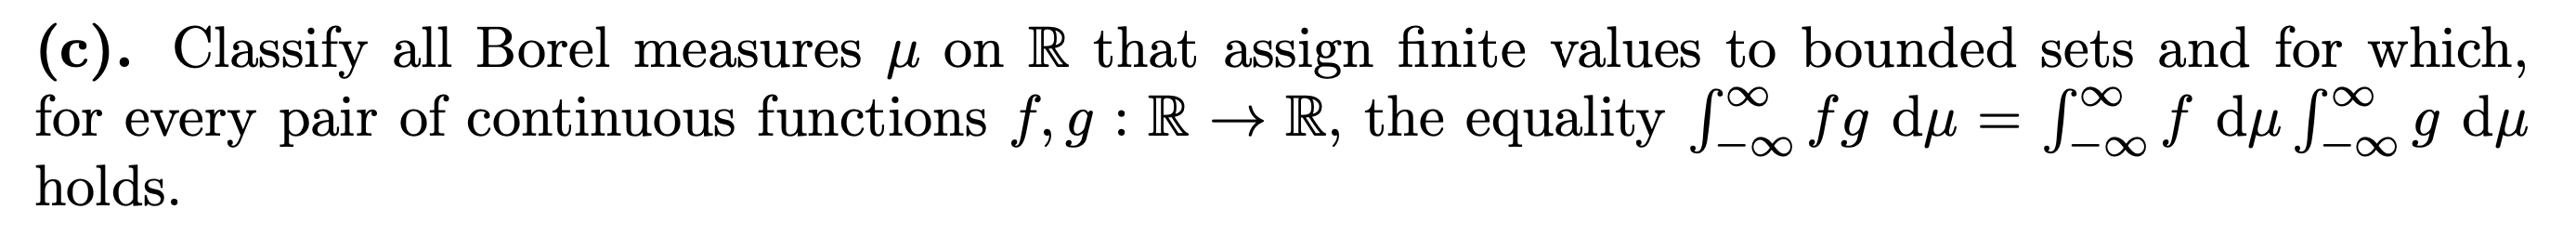
\includegraphics[width=400pt]{img/analysis--berkeley-202a-final-0bf8.png}
\end{mdframed}

% https://math.stackexchange.com/questions/2250993/when-the-integral-of-products-is-the-product-of-integrals

\begin{proof}
  \red{TODO}
  (No idea)
\end{proof}

\newpage
\begin{mdframed}
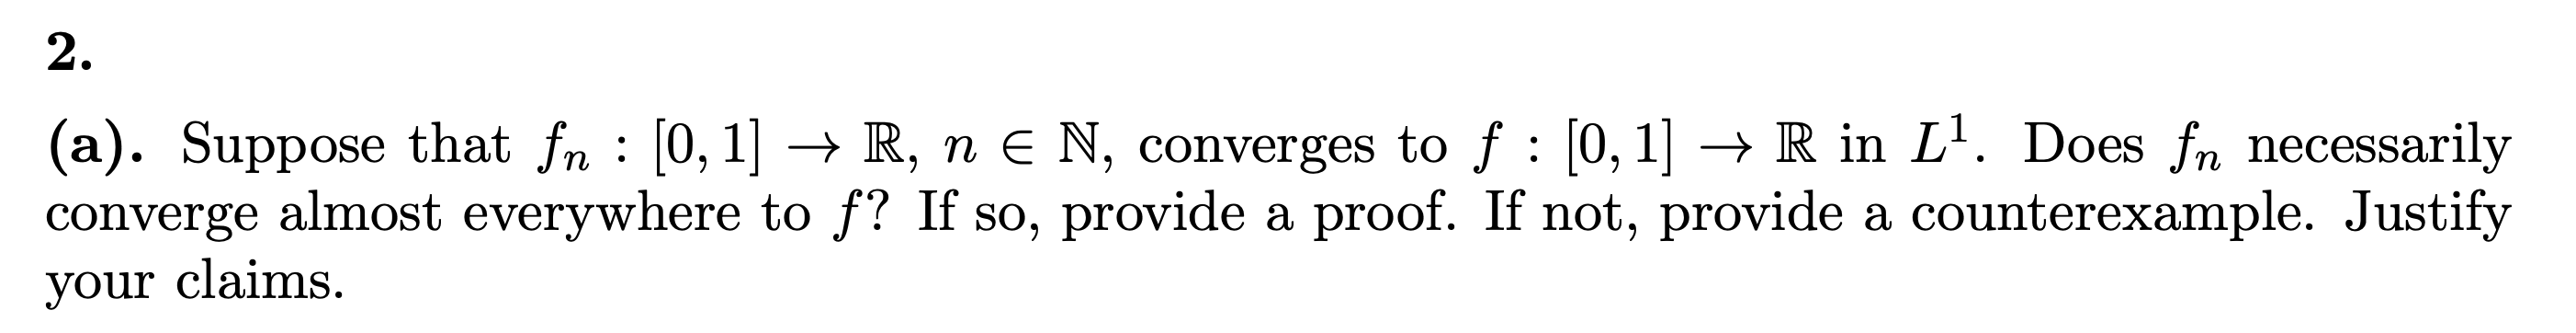
\includegraphics[width=400pt]{img/analysis--berkeley-202a-final-04b9.png}
\end{mdframed}

\begin{proof}
  \green{DONE}
  $f_n$ does not necessarily converge almost everywhere to $f$. Bass Example 10.7 is a counter example. I'm
  just going to copy it here rather than type it out myself, but I did do some thinking about this before
  consulting external sources (below).
\begin{mdframed}
  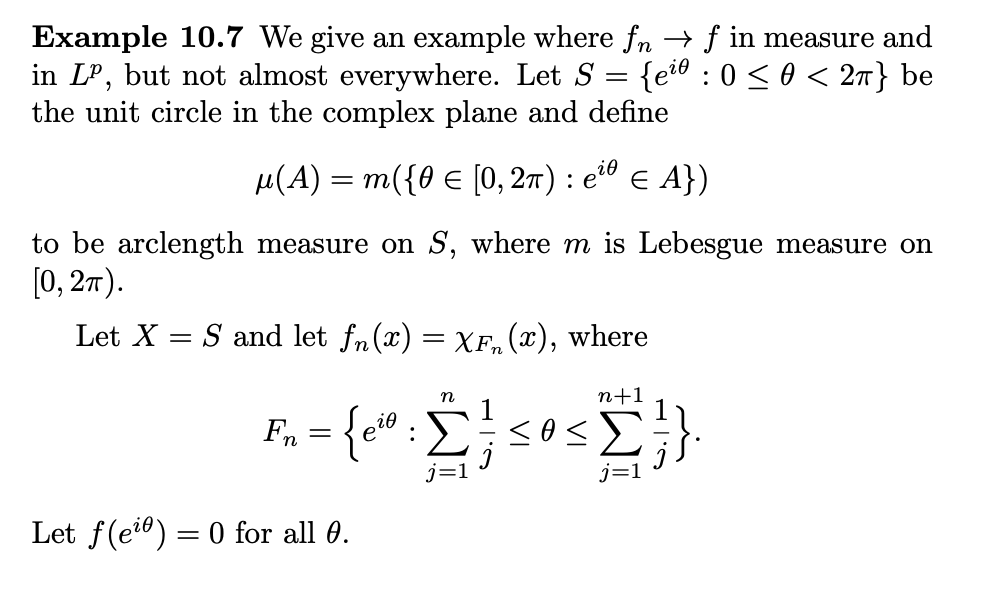
\includegraphics[width=400pt]{img/analysis--berkeley-202a-final-35f7.png}\\
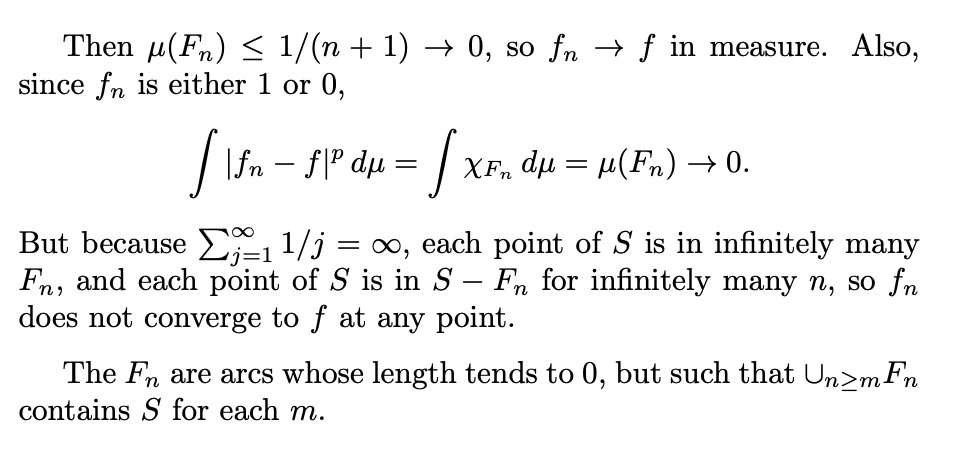
\includegraphics[width=400pt]{img/analysis--berkeley-202a-final-07d9.png}
\end{mdframed}
\end{proof}


\begin{proof}
  Let $f_n: [0, 1] \to \R$ be a sequence of functions converging to $f: [0, 1] \to \R$ in $L^1$.

  Let $E \subseteq [0, 1]$ be the set of points at which $f_n$ does not converge to $f$. Suppose for a
  contradiction that $\mu(E) > 0$.

  Since $f_n \to f$ in $L^1$ we have $\limninf \int |f_n - f| = 0$. Therefore $\limninf \int_E |f_n - f| = 0$.

  I think that's not possible and therefore a contradiction proving that $f_n \to f$ almost everywhere.

  (No, this is wrong -- see above)

  One might think that the sequences $f_n(x)$ for $x \in E$ could contrive to, at every generation $n$, almost
  all be exactly equal to $f(x)$, except for a negligible set, with membership of this negligible set changing
  over time such that every $x \in E$ will at some point in the future be a member of the error set again, in
  which case there would be convergence nowhere while retaining $\limninf \int_E |f_n - f| = 0$. However, if
  only a negligible set is allowed to participate at every generation $n$, then it is impossible for all the
  elements of a positive measure set to participate over the course of countably many generations.

  So it seems that this might be a contradiction, but we need to prove it.

  Set $d_n = |f_n - f|$ and let $\eps > 0$. Since $\int_E d_n \to 0$ there exists $N$ such
  that $\int_E d_n < \eps$ for all $n \geq N$. Let $n \geq N$.
\end{proof}

% \begin{theorem}[Bass proposition 8.1]\label{bass-8.1}
%   If $f$ is real-valued, non-negative, and measurable, and $\int f = 0$, then $f = 0$ a.e.
% \end{theorem}

% \begin{proof}
%   \red{TODO}
%   Let $f_n: [0, 1] \to \R$, $n \in \N$, converge to $f: [0, 1] \to \R$ in $L^1$. Thus, by definition,
%   \begin{align*}
%     \limninf \int |f_n - f| = 0.
%   \end{align*}
%   We want to prove or disprove the statement
%   \begin{align*}
%     \limn f_n = f \ae
%   \end{align*}
%   Suppose we could bring the limit inside. Then
%   \begin{align*}
%     \int \limninf |f_n - f| = 0,
%   \end{align*}
%   therefore by Bass proposition 8.1 $\limninf |f_n - f| = 0$ a.e. and thus $f_n$ converges almost everywhere to $f$.

%   But bringing the limit inside is justified by neither MCT nor DCT. So let's look for a counter-example based
%   on not satisfying DCT conditions.
% \end{proof}
I think my proof is put on a slightly firmer basis if I say at the outset that the syntax $e^{-x}$
is defined to mean the Maclaurin expansion: $e^{-x} := \sum_{j=0}^\infty (-1)^j ~ \frac{x^j}{j!}$.

\begin{lemma}\label{gamma-function}
  Define Euler's gamma function $\Gamma: \R \to \R$
  by $\Gamma(y + 1) = \int_0^\infty x^y e^{-x} \dx$ and note that integration by parts
  (with $u = x^n$, $\dvdx = e^{-x}$) yields
  \begin{align*}
    \Gamma(y + 1)
    &= \big[-x^ye^{-x}\big]_0^\infty + y\int_0^\infty x^{y-1}e^{-x} \dx \\
    &= y\Gamma(y),
  \end{align*}
  since $x^ye^{-x} \to 0$ as $x \to \infty$.

  Note that $\Gamma(1) = \int_0^\infty e^{-x} \dx = 1$, and therefore $\Gamma(n + 1) = n!$
  for $n \in \N$. (Since these are continuous functions, Lebesgue and Riemann integrals coincide
  and we freely use standard results for antiderivatives and derivatives from introductory
  calculus).
\end{lemma}

\begin{lemma}\label{exponential-limit}
  $(1 - x/k)^k < e^{-x}$ for all $k \in \N$ and all $x \in \R$
  and $\lim_{k \to \infty} \(1 - \frac{x}{k}\)^k = e^{-x}$.
\end{lemma}

\begin{proof}
  Recall the Maclaurin expansion $e^{-x} = \sum_{j=0}^\infty (-1)^j ~ \frac{x^j}{j!}$ and observe that
  \begin{align*}
    \(1 - \frac{x}{k}\)^k
    &= \sum_{j=0}^k {k \choose j} \(\frac{-x}{k}\)^j \\
    &= \sum_{j=0}^k (-1)^j \frac{x^j}{j!} \(\frac{k!/(k-j)!}{k^j} \) \\
    & <\sum_{j=0}^k (-1)^j \frac{x^j}{j!}.
  \end{align*}
  Therefore $(1 - x/k)^k < e^{-x}$ for all $k \in \N$ and all $x \in \R$.

  Furthermore we have
  \begin{align*}
    \lim_{k \to \infty} \(1 - \frac{x}{k}\)^k
    &= \sum_{j=0}^\infty (-1)^j \frac{x^j}{j!} \(\lim_{k \to \infty} \frac{k!/(k-j)!}{k^j} \).
  \end{align*}
  Note that
  \begin{align*}
    \lim_{k \to \infty} \frac{k!/(k-j)!}{k^j}
    &= \lim_{k \to \infty} \frac{k   (k - 1)     (k - 2)       \cdots (k - (j - 1))}{k^j} \\
    &= \lim_{k \to \infty} \frac{k^j (1 - k^{-1}) (k - 2k^{-1}) \cdots (1 - (j - 1)k^{-1})}{k^j} \\
    &= 1,
  \end{align*}
  therefore $\lim_{k \to \infty} \(1 - \frac{x}{k}\)^k = e^{-x}$.
\end{proof}

\begin{mdframed}
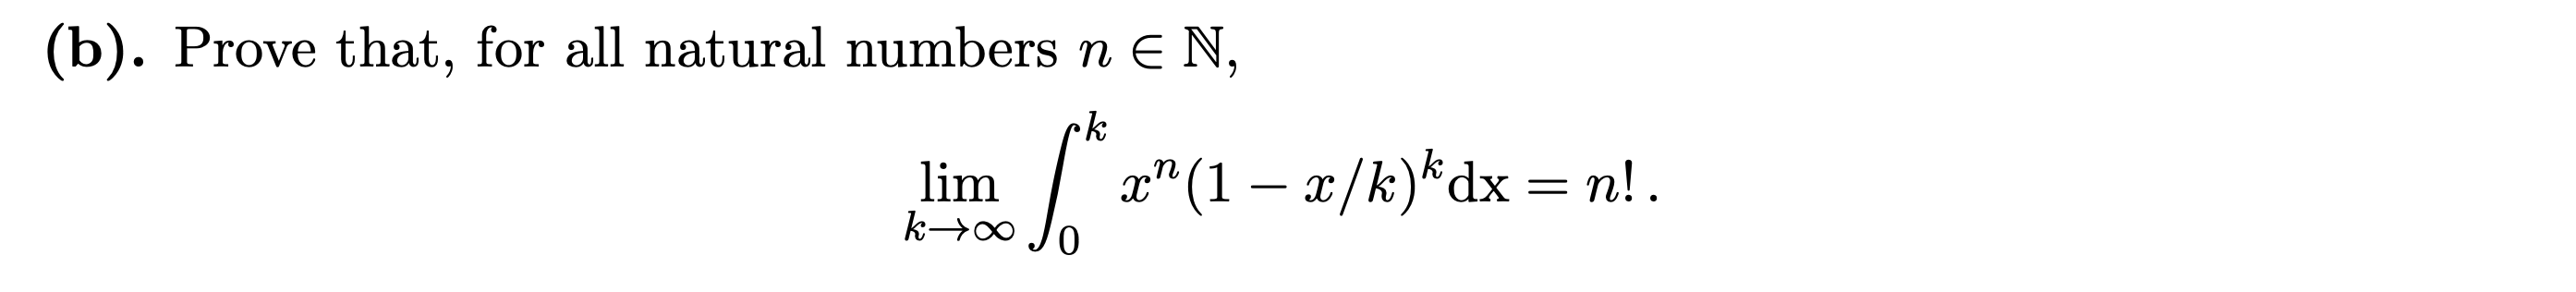
\includegraphics[width=400pt]{img/analysis--berkeley-202a-final-96cc.png}
\end{mdframed}

\begin{proof}
  \green{DONE}

  We may apply the dominated convergence theorem, since the integrand $x^n (1 - x/k)^k$ is
  non-negative and by lemma \ref{exponential-limit} is bounded above by $x^ne^{-x}$ which as shown
  in lemma \ref{gamma-function} is integrable.

  Therefore
  \begin{align*}
    \lim_{k \to \infty} \int_0^k x^n (1 - x/k)^k \dx
    &= \lim_{k \to \infty} \int_0^\infty x^n (1 - x/k)^k\ind_{[0, k]} \dx \\
    &= \int_0^\infty x^n \lim_{k \to \infty} (1 - x/k)^k\ind_{[0, k]} \dx & \text{by the dominated convergence theorem}\\
    &= \int_0^\infty x^n e^{-x} \dx & \text{by lemma \ref{exponential-limit}}\\
    &=: \Gamma(n + 1) \\
    &= n!  & \text{by lemma \ref{gamma-function}}.\\
  \end{align*}
\end{proof}

\red{TODO: What did this have to do with part (a)?}

\begin{mdframed}
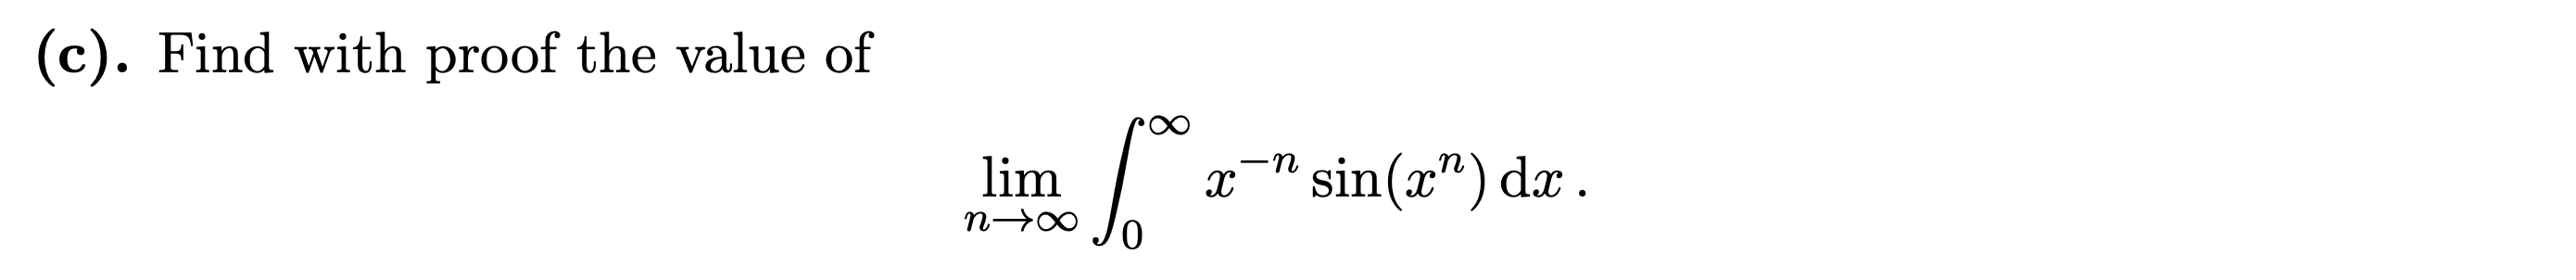
\includegraphics[width=400pt]{img/analysis--berkeley-202a-final-c137.png}
\end{mdframed}

\begin{proof}
  \red{TODO}
  bound the integral above?
\end{proof}


\newpage
\begin{mdframed}
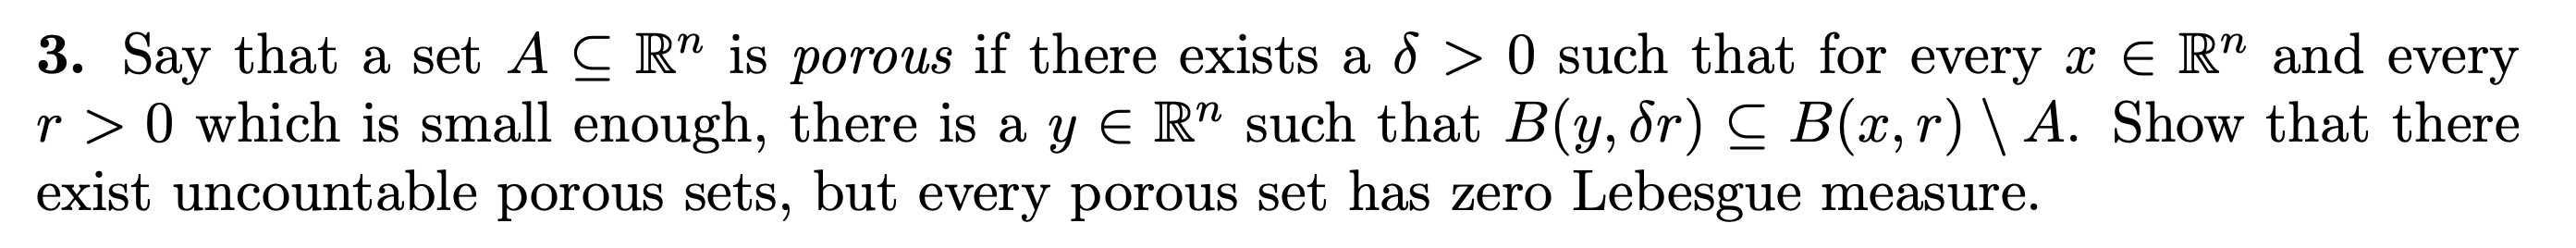
\includegraphics[width=400pt]{img/analysis--berkeley-202a-final-ef68.png}
\end{mdframed}

\begin{mdframed}
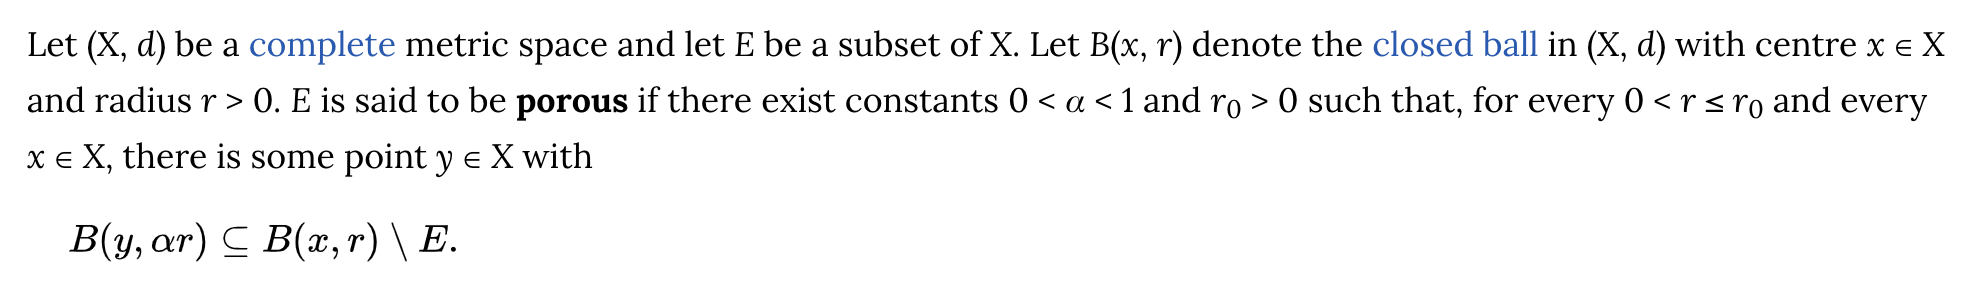
\includegraphics[width=400pt]{img/analysis--berkeley-202a-final-b463.png}
\end{mdframed}

Informally, here is what the definition says:

\begin{quote}
  For every ball (anywhere in $\R^n$) that is smaller than some fixed radius $r_0$, there exists an ``inner
  ball​'' that is smaller still by a factor of $\delta$, and which fits in the outer ball, while avoiding every
  point of $A$.
\end{quote}

Notice that in the definition, the same $\delta$ and $r_0$ work everywhere.

Consider an outer ball of size $r < r_0$. There exists an inner ball of size $\delta r$ that works. Furthermore
this inner ball works for all larger outer balls.

\begin{claim}
  There exist uncountable porous sets.
\end{claim}

\begin{proof}
  \green{DONE}

  Let $A = \R \times \{0\} \subset \R^2$. Note that $A$ is uncountable, since there is an obvious bijection
  between $A$ and the uncountable set $\R$.

  Take $\delta = 1/2$ and pick any $r_0 > 0$. Let $(x, y) \in \R^2$ and let $r < r_0$.

  Suppose $y \geq 0$. Then $B\big((x, y + r/2), r/2\big) \subset B\big((x, y), r\big)$
  and $B\big((x, y + r/2), r/2\big) \isect A = \emptyset$.

  Alternatively, suppose $y < 0$. Then $B\big((x, y - r/2), r/2\big) \subset B\big((x, y), r\big)$
  and $B\big((x, y - r/2), r/2\big) \isect A = \emptyset$.

  Therefore the uncountable set $A$ is porous.
\end{proof}

\begin{claim}
  Every porous set has zero Lebesgue measure.
\end{claim}

I used the following sources in answering this question

\url{https://www.wikiwand.com/en/Porous_set}\\
\url{https://math.stackexchange.com/questions/1362464/porous-sets-why-measure-zero}\\
\url{https://www.wikiwand.com/en/Lebesgue%27s_density_theorem}\\

\begin{proof}
  \red{TODO} (partial)

  Let $A \subseteq \R^n$ be porous, parametrized by $\delta > 0$ and $r_0 > 0$.

  Let $x \in A$ and let $y$ be such that for all $0 < r \leq r_0$ we have $B(y, \delta r) \subseteq B(x, r)$
  and $B(y, \delta r) \isect A = \emptyset$. Note that we have $m(B(y, \delta r)) < m(A^c \isect B(x, r))$.

  Now consider the ``density​'' $\frac{m(A \isect B(x, r))}{m(B(x, r))}$ of $A$ in $B(x, r)$. We have
  \begin{align*}
    \frac{m(A \isect B(x, r))}{m(B(x, r))}
    &= 1 - \frac{m(A^c \isect B(x, r))}{m(B(x, r))} \\
    &< 1 - \frac{m(B(y, \delta r))}{m(B(x, r))} \\
    &= 1 - \delta^n,
  \end{align*}
  where we have used the fact that the volume (and therefore the Lebesgue measure) of an $n$-ball of radius $r$
  is proportional to $r^n$.

  Suppose for a contradiction that $m(A) > 0$. Then by lemma \ref{lebesgue-density-theorem} (Lebesgue density
  theorem) we have that
  \begin{align*}
    \lim_{r \to 0} \frac{m(A \isect B(x, r))}{m(B(x, r))} = 1
  \end{align*}
  for Lebesgue-almost all points of $A$.

  \red{TODO} What exactly is the contradiction? This is certainly close to a contradiction.
  \red{TODO} Prove Lebesgue density theorem? E.g. from Folland 3.18?

  \red{Graders: Am I correct that the Lebesgue density theorem requires the set to have positive measure? It seems
    obviously true but I couldn't see that in statements of the result.}
\end{proof}



\newpage
\begin{mdframed}
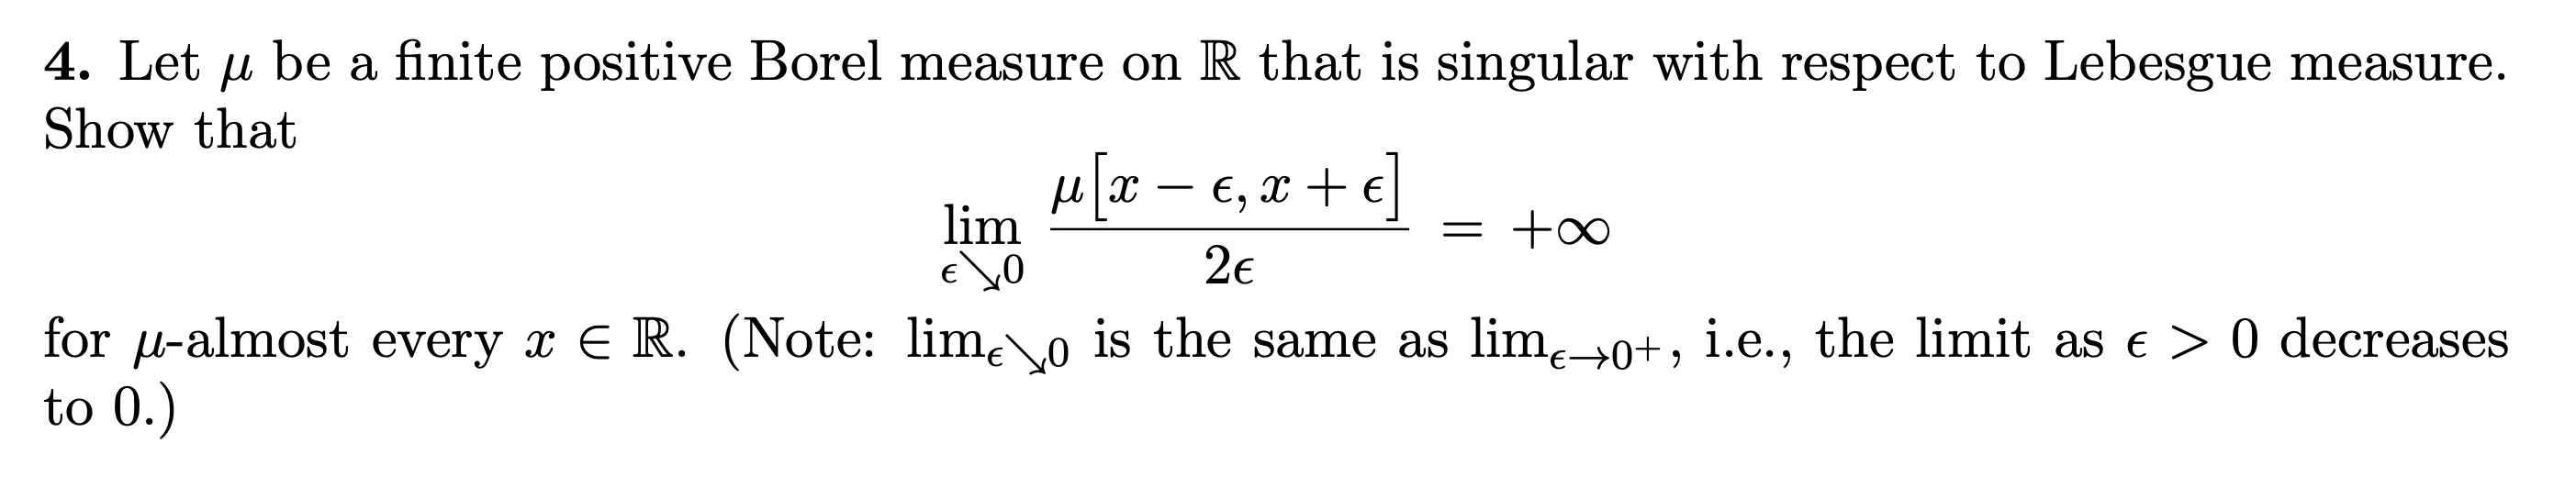
\includegraphics[width=400pt]{img/analysis--berkeley-202a-final-21a6.png}
\end{mdframed}

Let $m$ denote Lebesgue measure.

\begin{proof}
  \red{TODO} (partial)

  Since $\mu$ is singular with respect to Lebesgue measure, there exist disjoint Borel sets $U$ and $V$ such
  that $U$ is $\mu$-null and $V$ is $m$-null, and $\R = U \union V$.

  Let $0 < \mu(\R) = L < \infty$. We have
  \begin{align*}
    &\mu(U) = 0     & \mu(V) = L \\
    &m(U) = \infty & m(V) = 0,
  \end{align*}
  since by countable additivity $\infty = m(\R) = m(U) + m(V) = m(U)$,
  and $L = \mu(\R) = \mu(U) + \mu(V) = \mu(V)$.

  Note that any property that holds for all $x \in V$ holds $\mu$-almost everywhere. So let $x \in V$. We would
  like to show that
  \begin{align*}
    \lim_{\eps \searrow 0} \frac{\mu([x - \eps, x + \eps])}{2\eps} = +\infty.
  \end{align*}
  Let $\eps_n$ be a sequence converging to zero from above, let $I_n = [x - \eps_n, x + \eps_n]$, and
  let $B > 0$. We would like to show that there exists $N$ such that $\frac{\mu(I_n)}{2\eps_n} > B$ for
  all $n \geq N$.

  We have $\mu(I_n) = \mu(I_n \isect V) + \mu(I_n \isect U) = \mu(I_n \isect V)$, since $U$ is a null set
  under $\mu$. And since $x \in V$ we have $I_n \isect V \neq \emptyset$.

  If we could show that $\mu$-almost every singleton set included in $V$ has positive measure under $\mu$ then
  we would be done, since the property would hold at all of them. I think if we could show $V$ were countable
  then we'd be done for this same reason. But we can't -- e.g. the Cantor set has zero Lebesgue measure and yet
  is uncountable.

  Similarly, if we could show that there exists $N$ and $l > 0$ such that $\mu(I_n) > l$ for all $n > N$ then
  we would be done.

  Note that every interval around $x$ is not in $V$, because it has positive Lebesgue measure. In other
  words, $V$ includes no intervals. But this is true of the Cantor set also.

  My intuition is that as the interval $I_n$ gets smaller, it becomes enriched for points of $V$, which
  contribute positive measure to the numerator, and cause it to decrease more slowly than the denominator, in
  such a way that, for small enough $\eps$, the ratio exceeds any positive quantity $B$.

  \red{TODO} Finish this.
\end{proof}

% I am assuming that the question is saying that $\mu$ and $m$ are mutually singular with respect to the
% Borel $\sigma$-algebra.

% Intuition: in some sense this question is asking us to show that the Radon-Nikodym derivative does not exist,
% because they are singular, which is sort of the opposite of absolutely continuous.

% Intuition: $\mu$ assigns positive measure to a $m$-null set. Clearly we need to show that $\mu$ assigns greater
% measure to certain intervals than $m$ does. Why is that true? Perhaps because the interval contains parts of
% an $m$-null set.

% In fact, $\mu$ only has positive measure on Lebesgue null sets. But $\mu$ does not assign positive measure to
% every singleton, since $\mu$ is finite. If we could show that $\mu$-almost every $x$ is ``surrounded by an
% arbitrarily small Lebesgue null set​'' that would do it. Perhaps the only way that makes sense is if
% $\mu$-almost every $x$ is a singleton with positive measure under $\mu$. Can we show that?

% $V$ contains no intervals, since it is Lebesgue-null. And $\mu(V) = L > 0$. This total measure $L$ is assigned
% to Lebesgue-null sets in a countably additive manner.

% \begin{mdframed}
% 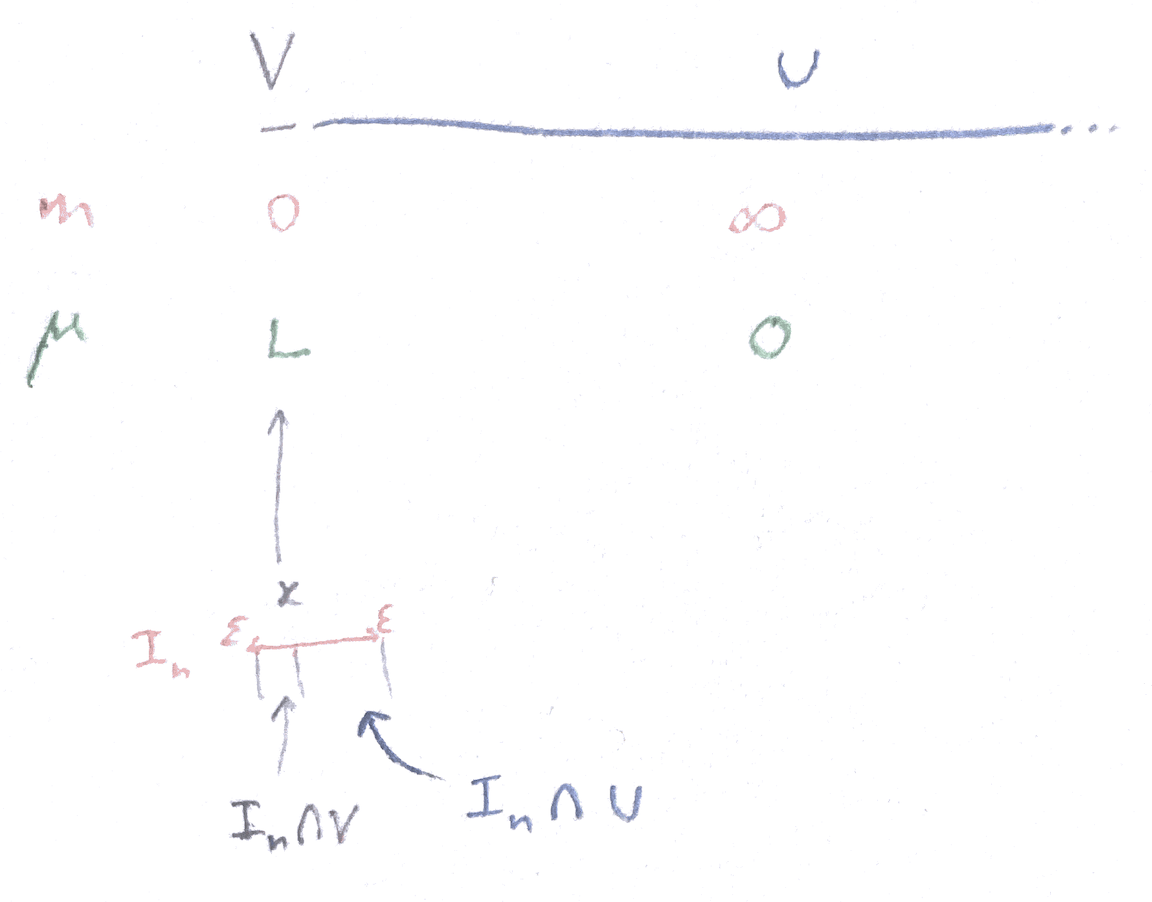
\includegraphics[width=200pt]{img/analysis--berkeley-202a-final-fe0f.png}
% \end{mdframed}



\newpage
\begin{mdframed}
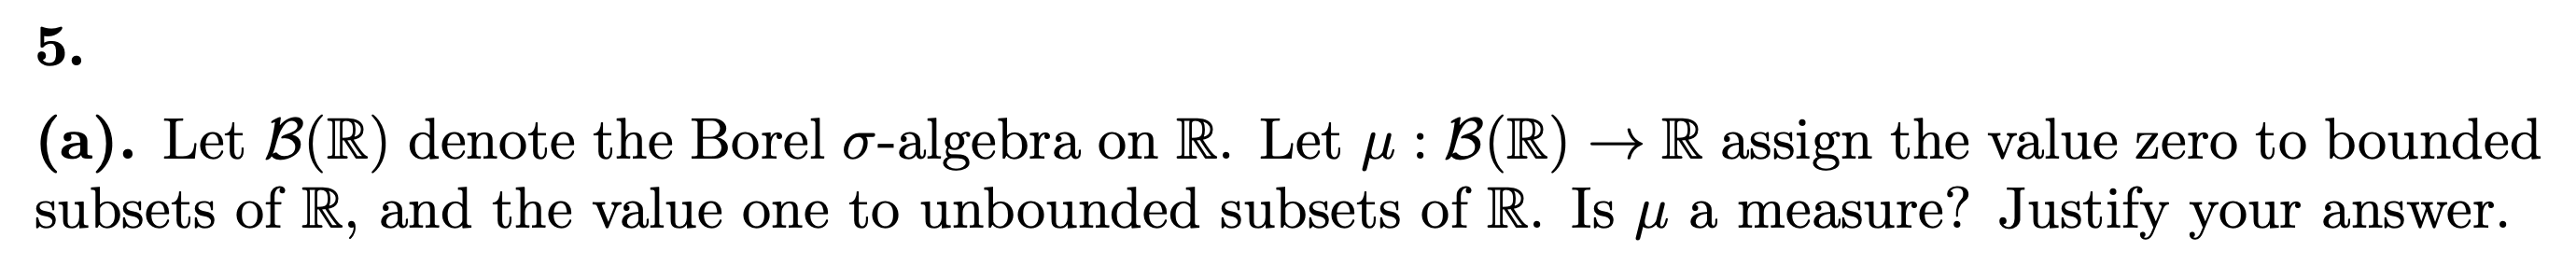
\includegraphics[width=400pt]{img/analysis--berkeley-202a-final-246a.png}
\end{mdframed}

\begin{proof}
  \green{DONE}

  $\mu$ is not a measure because it is not countably additive.

  To see this, let $I_n = (-n, -(n - 1)] \union [n-1, n)$, and let $\mc I = \{I_n ~:~ n \in \N\}$. Then $\mc I$
  is a pairwise disjoint, countable collection of sets and $\bigcup_{n=1}^\infty \mc I = \R$,
  therefore $\mu\(\bigcup_{n=1}^\infty \mc I\) = 1$ since $\R$ is unbounded.

  However $I_n$ is bounded for all $n$ and
  so $\sum_{n=1}^\infty \mu(I_n) = \sum_{n=1}^\infty 0 = 0 \neq \mu\(\bigcup_{n=1}^\infty \mc I\)$.
\end{proof}


\begin{mdframed}
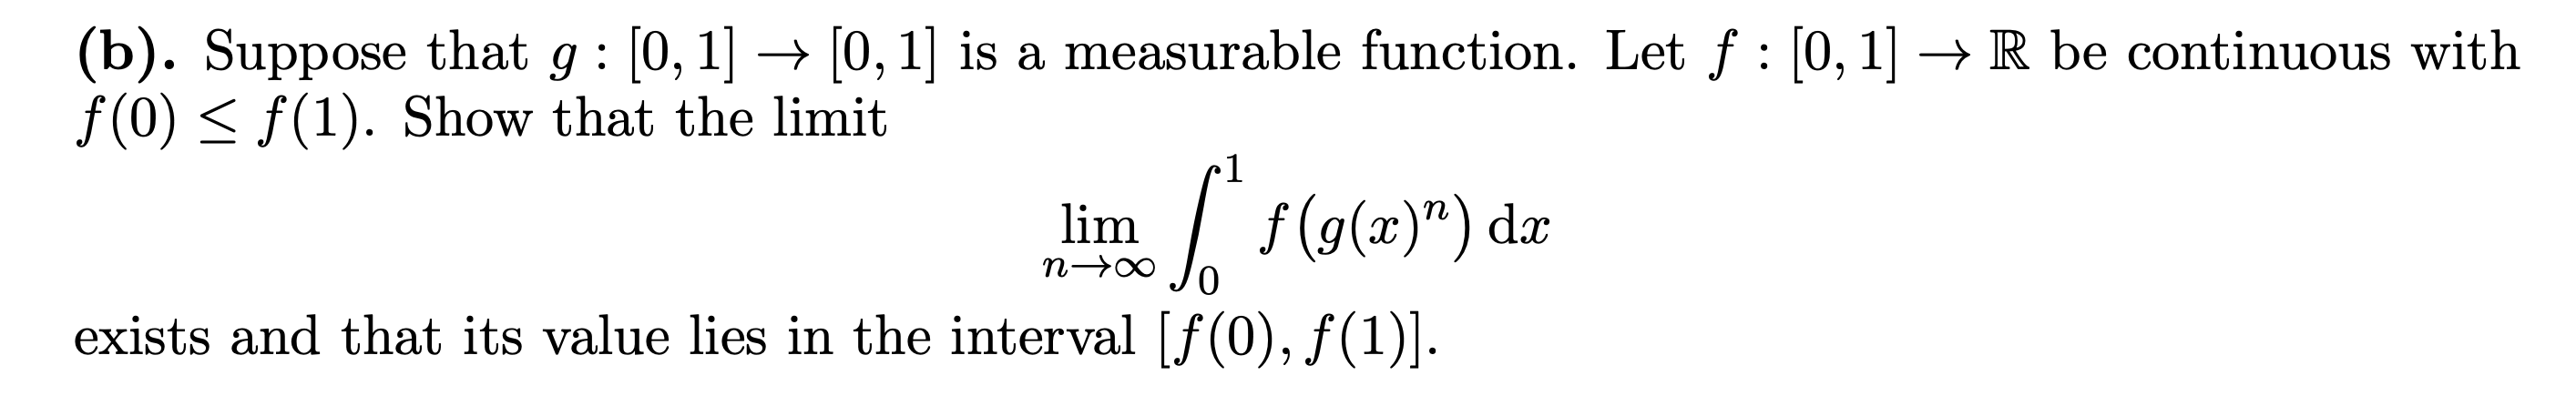
\includegraphics[width=400pt]{img/analysis--berkeley-202a-final-cd70.png}
\end{mdframed}

\begin{proof}
  \green{DONE}

  Note that $f$ is continuous with compact support and so $f$ attains its bounds. Let $A = \inf f$
  and $B = \sup f$.

  Note that the integrand is bounded above by the constant integrable function $h(x) = B$ defined on $[0, 1]$.
  Therefore we may apply the dominated convergence theorem, yielding
  \begin{align*}
    \limninf \int_{[0, 1]} f(g(x)^n) \dx = \int_{[0, 1]} \limninf  f(g(x)^n) \dx.
  \end{align*}
  Let $U = g^{-1}(\{1\})$. We have $0 \leq g(x) \leq 1$ and therefore
  \begin{align*}
    \limninf g(x)^n =
    \begin{cases}
      1 & x \in U \\
      0 & \text{otherwise}.
    \end{cases}
  \end{align*}
  Since $g$ is measurable, $U$ is measurable, since it is a preimage of a measurable set. Let $\alpha = m(U)$.
  I believe that ``measurable​'' in the question refers to Lebesgue measure, so we have that $m([0, 1]) = 1$
  and $0 \leq \alpha \leq 1$. Therefore
  \begin{align*}
    \int_{[0, 1]} \limninf  f(g(x)^n) \dx
    &= \int_U \limninf  f(g(x)^n) \dx + \int_{[0, 1] \setminus U} \limninf  f(g(x)^n) \dx \\
    &= \int_U f(1) + \int_{[0, 1] \setminus U} f(0) \\
    &= \alpha f(1) + (1 - \alpha) f(0) \\
    &\in [f(0), f(1)].
  \end{align*}
\end{proof}


\newpage
\begin{mdframed}
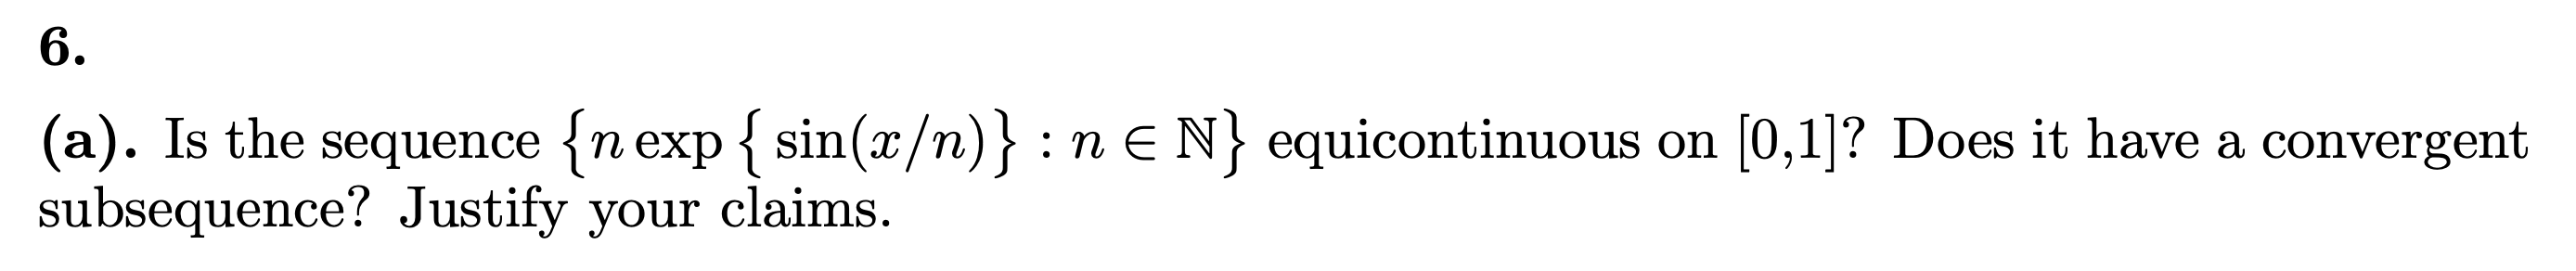
\includegraphics[width=400pt]{img/analysis--berkeley-202a-final-f5b6.png}
\end{mdframed}

\begin{proof}
  \red{TODO}

  My intuition is that this will not be equicontinuous because of the way that $x/n$ is changing the frqeuency
  of the sine curve.

  I believe we have to agree on a norm/metric for this function space. I will assume this is $L^1$, i.e. $d(f, g) = \int |f - g|$.

  In a compact subset of a metric space, every sequence has a convergent subequence. Is this set of functions compact in $L^1$?
\end{proof}

\begin{mdframed}
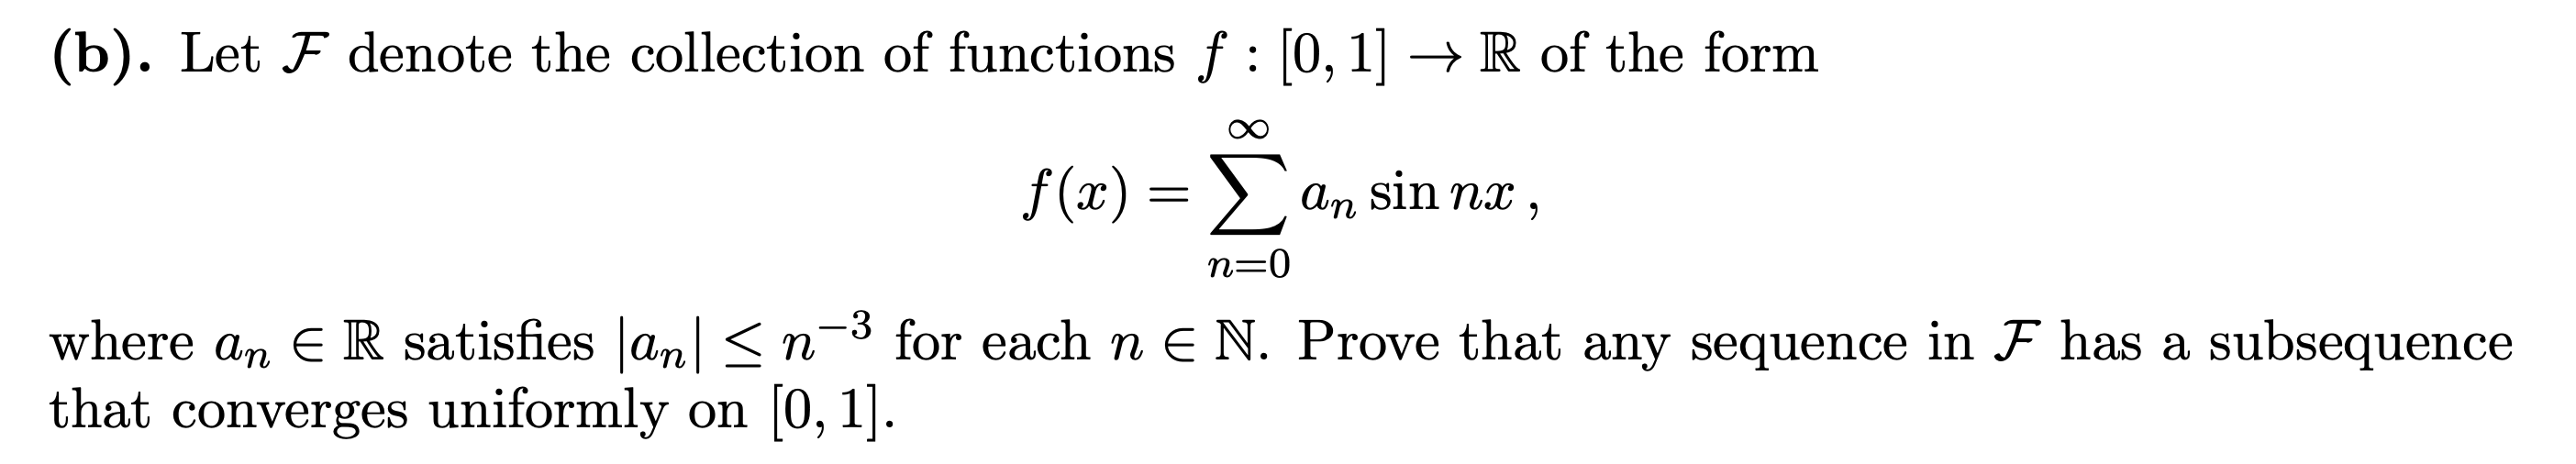
\includegraphics[width=400pt]{img/analysis--berkeley-202a-final-c7c7.png}
\end{mdframed}

% https://math.berkeley.edu/~vvdatar/m104su18/Assignments/Solutions_A7.pdf

\begin{proof}
  \red{TODO}

  By the Ascoli - Arzelà theorem, $\mc F$ has a subsequence that converges uniformly on $[0, 1]$ if the
  following two conditions are met:
  \begin{enumerate}
  \item  $\origsup_{f \in \mc F} |f(x)| < \infty$ for all $x \in [0, 1]$
  \item $\mc F$ is equicontinuous.
  \end{enumerate}
\end{proof}


\newpage
\begin{mdframed}
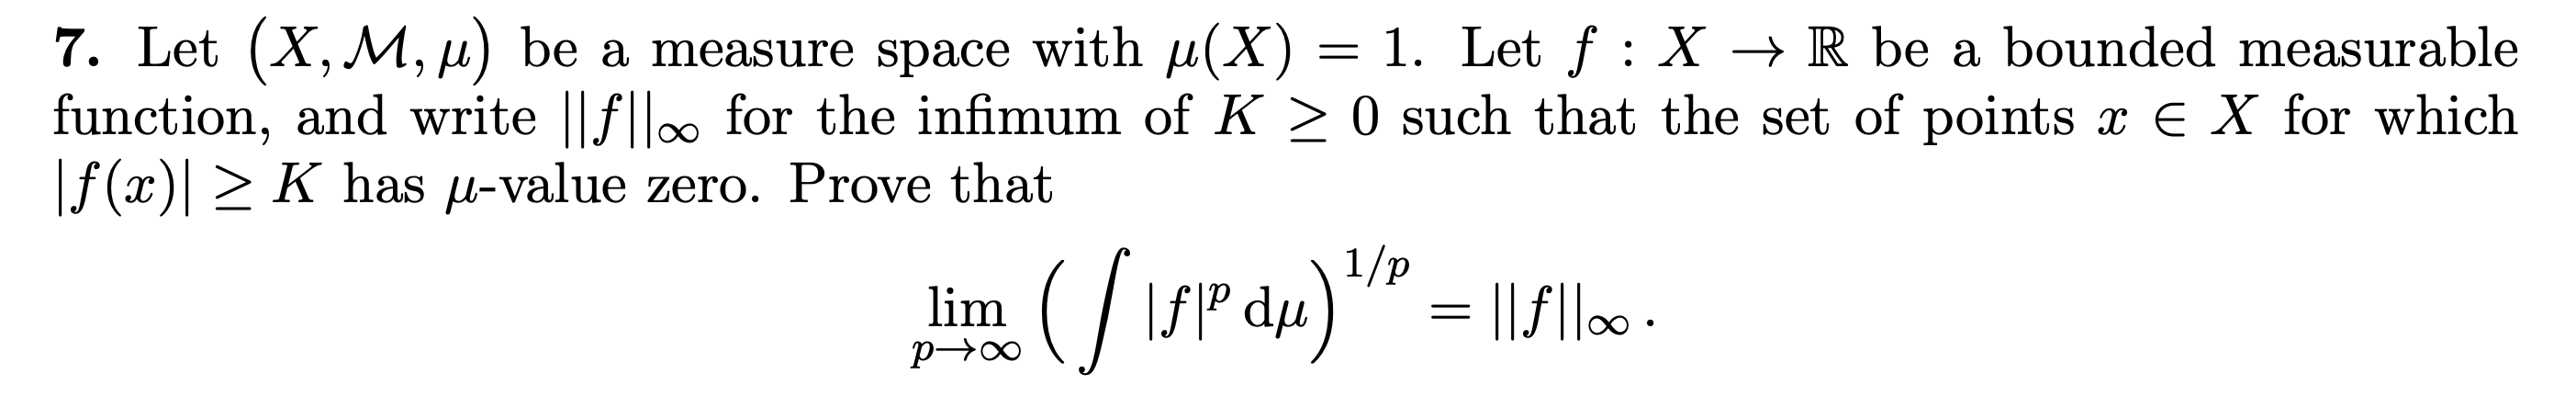
\includegraphics[width=400pt]{img/analysis--berkeley-202a-final-0000.png}
\end{mdframed}


My first thought was to attempt to prove this by proving it for $f$ simple, then for $f$ measurable, etc. But I
have now seen the following resources and am submitting a proof based on them.

\url{https://www.wikiwand.com/en/Lp_space#/The_p-norm_in_infinite_dimensions_and_%E2%84%93p_spaces}\\
\url{https://www.wikiwand.com/en/Essential_supremum_and_essential_infimum}\\
\url{https://math.stackexchange.com/questions/242779/limit-of-lp-norm}\\
\url{https://math.stackexchange.com/questions/678884/if-f-in-l-infty-and-exists-r-infty-so-that-f-r-infty-show?noredirect=1&lq=1}\\


\begin{proof}
  \red{TODO} (partial)
  Let $\norm{f}_p = \(\int |f|^p \dmu\)^{1/p}$.

  First we will prove that $\norm{f} \leq \norm{f}$.

  Let $\eps > 0$, and define $E_\eps := \{x \in X ~:~ |f(x)| \geq K - \eps\}$. Then we have
  \begin{align*}
    \int |f|^p \dmu \leq \int_{E_\eps} |f|^p \dmu
  \end{align*}
\end{proof}

Here is the proof I started attempting before looking at any other sources:

\begin{proof}

  [incomplete]

  Let $L = \lim_{p \to \infty} \(\int |f|^p \dmu\)^{1/p}$.

  First consider $f$ simple, say $f = \sum_{j=1}^J a_j \ind_{E_j}$. Then
  \begin{align*}
    \int |f|^p \dmu = \sum_{j=1}^J |a_j|^p \mu(E_j)
  \end{align*}
  and (\red{TODO} proof)
  \begin{align*}
    \lim_{p \to \infty} \(\int |f|^p \dmu\)^{1/p}
    &= \max \Big\{|a_j| ~:~ \mu(E_j) > 0, j \in \{1, \ldots, J\}\Big\} \\
    &= \norm{f}_\infty.
  \end{align*}
  Next, consider $f$ measurable. Let $s_n$ be a sequence of simple functions increasing to $f$. Then
  \begin{align*}
    \int |f|^p \dmu = \lim_{n \to \infty}\sum_{j=1}^{J_n} |a_{nj}|^p \mu(E_{nj})
  \end{align*}

  First we will show that $L \geq \norm{f}_\infty$.

  Finally we show that $L \leq \norm{f}_\infty$.
  \red{TODO}
\end{proof}


Let $A = \originf_{x \in X} f$ and let $B = \origsup_{x \in X} f$. Since $f$ is bounded these are both
finite.

Since $f$ is bounded, $|f|$ is bounded also. Let $B = \origsup_{x \in X} |f(x)|$. We
have $\norm{f}_\infty \leq B$.



As an example, let $f(x) = 0.9$ for all $x \in X$.
Then $\(\int |f|^p \dmu\)^{1/p} = \(0.9^p\int 1 \dmu\)^{1/p} = 0.9$, so that is as expected.


\newpage
\begin{mdframed}
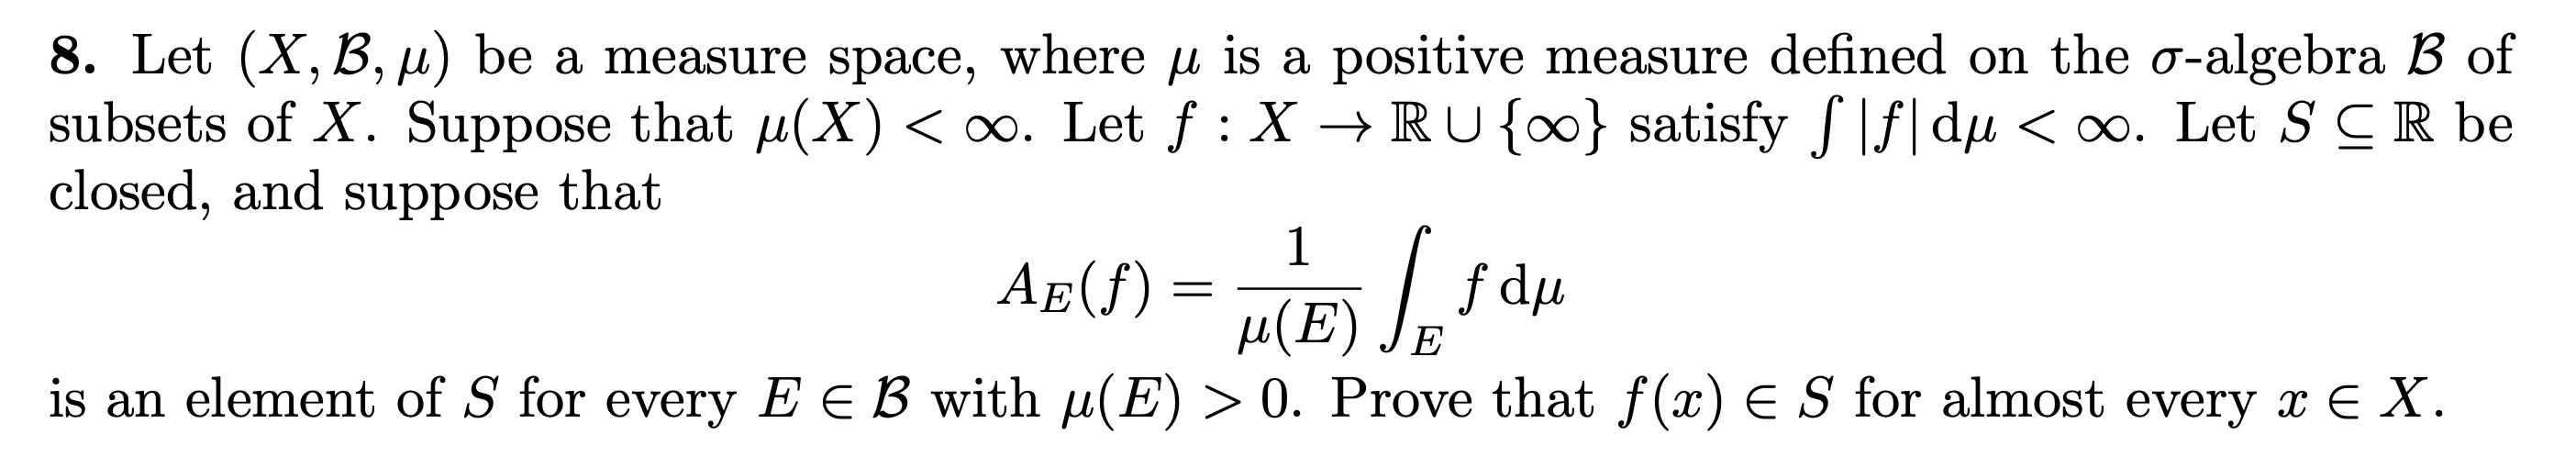
\includegraphics[width=400pt]{img/analysis--berkeley-202a-final-8aed.png}
\end{mdframed}

This question involves an averaging construction similar to that associated with Hardy-Littlewood maximal
function theory and the Lebesgue differentiation theorem (Folland section 3.4). However, the theory in Folland
3.4 concerns $\R^n$, whereas this question is about an abstract measure space. It doesn't look like extensions
of that theory to abstract measure spaces are well-known, or at least not standard graduate-level material.
Wikipedia (\url{https://en.wikipedia.org/wiki/Lebesgue_differentiation_theorem}) mentions that the Lebesgue differentiation theorem holds for a
``finite Borel measure on a separable metric space​'' obeying certain conditions and references Federer 1969, but
we don't have that.

We are however given a finite measure space $\mu(X) < \infty$; that may be a clue. Also we have a measurable
function to $\R \union \{\infty\}$. I wonder whether we can transfer some of the results over from $\R^n$
somehow.


\begin{proof}
  \red{TODO}
  If $\mu(X) = 0$ then the result is trivially true so we assume $\mu(X) > 0$.

  We would like to show that for almost every $x$ a sequence of sets $E_n$ exists, each of positive measure,
  such that $A_{E_n}(f) \to f(x)$. Then, since $S$ is closed, it contains the limit of every convergent
  sequence in $S$, and hence we would have $f(x) \in S$ for every $x \in X$.

  \begin{itemize}
  \item We must use that $\mu(X) < \infty$.
  \item We must use that $\int |f| \dmu < \infty$.
  \item We are asked only for almost every $x \in X$
  \end{itemize}
\end{proof}

\begin{proof}
  \red{TODO} No, this is wrong. The measure space is not necessarily $\R^n$.

  Since $f$ is integrable, it is locally integrable. So from Folland 3.18 we have
  that $\lim_{r \to 0} A_{B(x, r)}(f) = f(x)$ for a.e. $x \in \R$. Let $x$ be such a point and
  let $I^{(x)}_n = [x, x + 1/n)$ and note that $\limninf I^{(x)}_n = \{x\}$ and that $I^{(x)}_n \in \mc B$ for
  all $n$.

  Thus $A_{I^{(x)}_n}$ is a sequence in $S$. We would like to show (\red{TODO}) that this sequence converges
  to $f(x)$. Then, since $S$ is closed, it contains the limit of every convergent sequence in $S$,
  hence $f(x) \in S$ for almost every $x \in X$.

  \red{TODO} However, what we need to address is that $A_{\{x\}}(f)$ is not defined, since $\mu(\{x\}) = 0$. It
  certainly seems plausible that $A_{I^{(x)}_n} \to f(x)$, but we need to prove it. Perhaps this is related to
  Lebesgue density results.
\end{proof}
